\chapter{Introduction}
\label{chap:introduction}
One of the fundamental concepts to teach in a database design course is 
relation decomposition, which consists of dividing relations (or data tables) into smaller
tables in order to reduce redundancy, eliminate wasted storage, and more importantly reduce
anomalies or inconsistencies due to data updates. The central tool in producing these
decompositions and refinement of the database into what is called normal forms 
is the normalization theory. 
Unfortunately, theory is not yet understood well by practitioners~\cite{p1}.
One of the reasons for this is the lack of good tools which could aid the students 
during the learning process of relational-database normalization~\cite{p8}. 
Thus our learning environment was developed at the Ume� University 
as the core of a previous thesis~\cite{mt1}. 
It gives students the ability to easily and efficiently test
their knowledge of the different normal forms in practice. The environment assists the students by 
providing them with the following functionalities:

\begin{enumerate}
	\item Allow the student to specify a candidate decomposition of a given relation.
	\item Assess the correctness of the student's proposed decomposition relative to many factors; including:
		\begin{itemize}
			\item Lossless-join property.
			\item Dependency preservation.
			\item Specification of keys.
			\item Correctness of the Second Normal Form (2NF), Third Normal Form (3NF) and
			 Boyce-Codd Normal Form (BCNF) decompositions.
		\end{itemize}
	\item Provide students with sample decompositions when needed. 
	\item Allow users to communicate with each other via comments/posts.
\end{enumerate}



\section{Organization of this Report}
\label{sec:organization}
In the remaining sections of this chapter we introduce informally 
the key features and concepts of our Web-based learning environment, 
called LDBN (Learn DataBase Normalization)~\cite{wldbn}; 
compare it to a couple of other 
available Web-based database normalization tools, and provide the reader with small glossary.  
%The introduction to LDBN in Section~\ref{sec:introldbn} is important for the reader
%in order for him/her to better understand the need and the concepts of the algorithms described in 
In Chapter~\ref{chap:motivation} we present some of the issues we encountered during the testing period
of the system. 
In Chapter~\ref{chap:approach} we discuss some design issues regarding LDBN such as 
platform choice and others and present our implementation.  
Chapter~\ref{chap:conclusion} shows our conclusions.

\section{Learning Database Normalization with LDBN}
\label{sec:introldbn}
In this section we briefly introduce our reference implementation
of the Web-based learning environment, called LDBN.
It should be noted that discussing the system in detail is beyond the scope of this report. 
However, a formal overview of the system can be found in~\cite[Chapter~1 and Chapter~4]{mt1}.

Figure~\ref{fig:screen01} shows the overview of the most important part of the 
user interface~(UI)~- 
the \textit{Solve Assignment} view/tab. Here students can test their knowledge on 
the subject of relational-database normalization. The first thing the reader 
may notice is the fact that LDBN runs within a Web browser. The client side 
of LDBN is written in JavaScript following the AJAX techniques 
(more about this in Section~\ref{sec:platform}). 
Furthermore, LDBN is assignment driven. This means students have to first 
choose an assignment 
from a list with assignments, submitted by other users (lecturers). 
An assignment consists of a relational-database schema in
universal-relation form (URF), i.e., all the attributes in a single relation 
and a set of FDs on the attributes. 
After an assignment has been loaded, we require the students to go through the 
following steps in LDBN:
\begin{enumerate}
	\item Determine a minimal cover of the given FDs, also known as a canonical cover.
	\item Decompose the relational schema which is in URF into 2NF, 3NF and BCNF. 
	\item Determine a primary key for each new relation/table. 
\end{enumerate}

The task of checking a potential solution
involves many subtasks, which may be performed in any order. In addition to this,  
a partial or complete 
solution can be submitted at any given time by pressing the \textit{Check Solution} button. 
After that the system analyzes the solution by performing series of tests, which are not
discussed here since implementing those tests was not part of this thesis. 

A dialog with the result is shown to the user. In case of an error the system offers
feedback in form of small textual hints, indicating
where the error might be. 

\begin{figure}[h]
	\begin{center}
		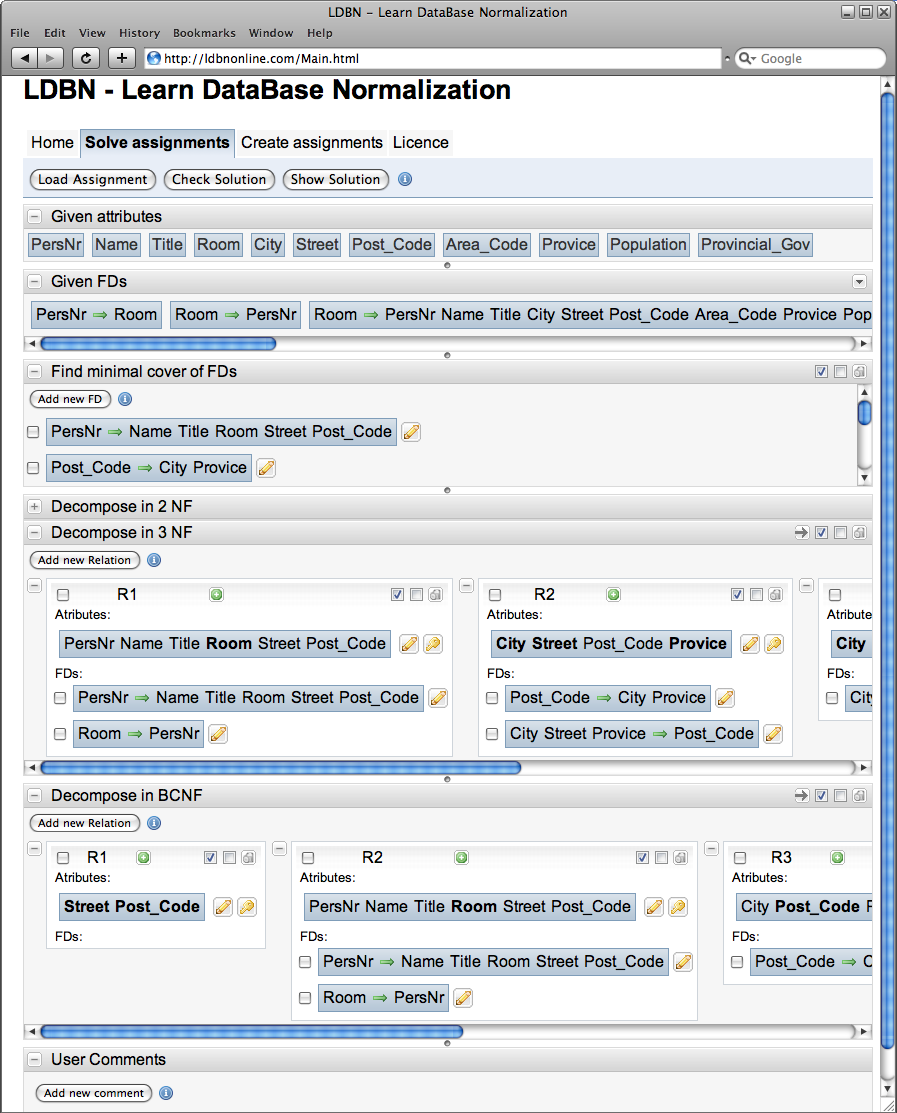
\includegraphics[width=0.84\textwidth]{./img/screen01b.png}
		\caption{Solve Assignments Tab}
		\label{fig:screen01}
	\end{center}
\end{figure}

Additional features of LDBN include creating an assignment, which can be done 
only by registered users, i.e., users who have filled out a registration form and their email
has been confirmed by the system. These users can log-in into the system with their user name and password 
and use additional features of the system.  At this point it should be mentioned that
there are different types of registered users with different rights and privileges in the systems 
and only the assignments submitted by instructional users (lecturers) are visible by default, but a user can
choose to see all assignments. This restriction is necessary in order users to be able 
to distinct assignments provided by trusted users, e.g., the database course
lecturers. Registered users have also the ability to leave textual comments 
for every assignment. On the one hand, such
comments ensure that user can easily communicate and share ideas
with each other, and one the other hand, comments could also decrease the amount of workload
for the lecturers in terms of giving an explanation to difficult decomposition.

%More detailed and formal description of the features of LDBN will be given in
%Chapter~\ref{chap:motivation}. 

\section{Glossary}
\begin{description}
	\item[2NF, 3NF, BCNF] \emph{Second Normal Form, Third Normal Form, Boyce-Codd Normal Form}. 
	  Discussing the different normal forms, the relational  data model and the relational-database normalization
    is beyond the scope of this report. 
	  For readers who are unfamiliar with subject of normal forms and relational-database
    normalization we recommend the textbook by Elmasri and Navathe~\cite{bdb1} or
    the textbook by Kemper and Eickler~\cite{bdb2} for German-speaking readers, both of which have 
    proven to be helpful guides throughout the development process of LDBN. 
    In addition to those, there are many free on-line resources such as the article 
    \emph{A Simple Guide to Five Normal Forms in Relational Database Theory} by Kent~\cite{p7}. 
    There is also a brief introduction to relational-database normalization in ~\cite[Chapter~2]{mt1}.
	\item[AJAX] \emph{Asynchronous JavaScript And XML} 
	  Asynchronous JavaScript And XML is a group of interrelated Web development techniques 
	  used for creating interactive Web applications, for more details see Section~\ref{sec:platform}.
	\item[API] An \emph{Application Programming Interface} is a set of functions, procedures or classes 
	  that an operating system, library or service provides to support requests
	  made by computer programs~\cite{wapi}.
	\item[CSS] \emph{Cascading Style Sheets} is a style sheet language used to describe the 
	  presentation of a document written in HTML.
	\item[DBMS] A \emph{Database Management System} is a complex set of software programs that
	  controls the organization, storage, management, and retrieval of data in a database.
	\item[FD] A \emph{functional dependency (FD)} is a constraint between two sets of 
	  attributes in a relational database. Additional details may be found in~\cite{bdb1}, 
	  \cite{bdb2}, \cite{p7}, or \cite[Chapter~2]{mt1}.  
	\item[GWT] \emph{Google Web Toolkit} is an open source Java software development 
	  framework that allows Web developers to create AJAX applications in Java. 
	  Additional details may be found in Section~\ref{sec:gwt}.
	\item[LDBN] \emph{Learn Database Normalization} 
	  is our reference implementation of the Web-based environment for
    learning normalization of relational database schemata. We often refer to LDBN 
    as \emph{our learning environment} or \emph{our implementation}. 
    We distinguish between two versions of LDBN - 
    the initial or original version described in~\cite{mt1}; and the improved version
    discussed in this report. In order for the reader to better distinguish between the two
    versions we also refer to the original version as LDBN 1.0, and to the improved version
    as LDBN 1.1.  
    The reference implementation of the system can be found at \url{http://ldbnonline.com}.
	\item[ODBC] \emph{Open Database Connectivity} provides a standard 
	  software API method for using database management systems.
%	\item[RPC] \emph{Remote Procedure Call} is an inter-process communication 
%	  technology that allows a computer program to cause a subroutine or 
%	  procedure to execute in another address space.
	\item[SQL] \emph{Structured Query Language} is a computer language designed for 
	  the retrieval and management of data in relational database management systems, 
	  database schema creation and modification, and database object access control management.
	\item[XMLHttpRequest] is an API that can be used by JavaScript and other Web browser 
	  scripting languages to transfer XML and other 
	  text data asynchronously between a Web server and a browser.
\end{description}
